\section{Эксперимент}

Собрав конструкцию получим:

\begin{figure}[h]
    \centering
    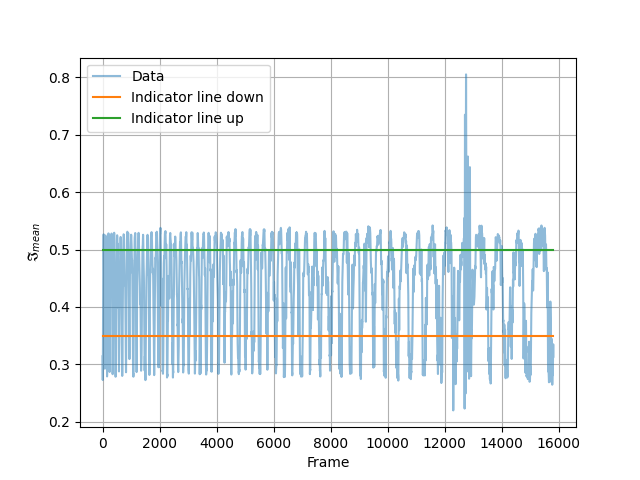
\includegraphics[trim={0 0 0 0},clip,width=\textwidth]{Ex_3/3_3.png}
    \caption{$T_0 = 28C, T_1 = 35C, n = 60$}
    \label{3_1}
\end{figure}

\begin{figure}[h]
    \centering
    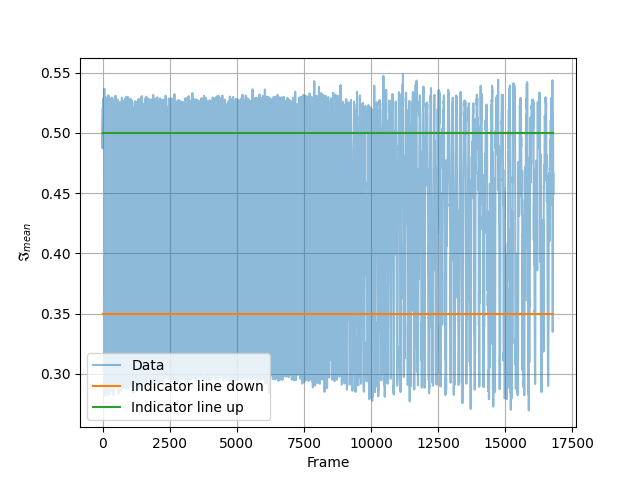
\includegraphics[trim={0 0 0 0},clip,width=\textwidth]{Ex_3/3_2.png}
    \caption{$T_0 = 35C, T_1 = 63C, n = 235$}
    \label{3_2}
\end{figure}

\begin{figure}[h]
    \centering
    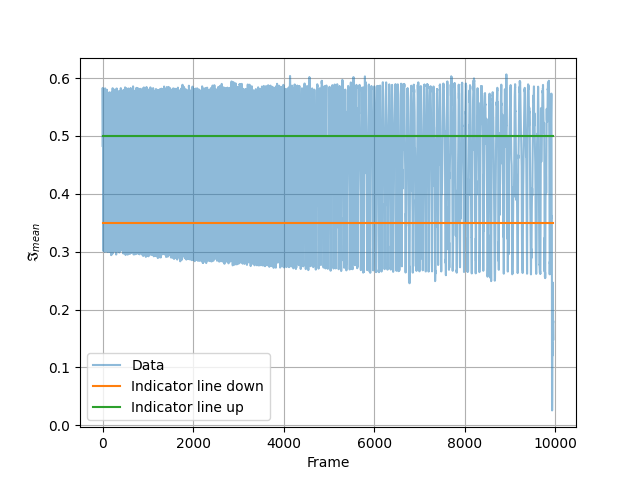
\includegraphics[trim={0 0 0 0},clip,width=\textwidth]{Ex_3/3_1.png}
    \caption{$T_0 = 63C, T_1 = 88C, n = 202$}
    \label{3_3}

\end{figure}



Пердположим что:
\begin{eqnarray}
    \Delta l = k \Delta T
\end{eqnarray}

Тогда по полученным данным
















